% Source: AESP_466_ClassWork/Assignments/Assignment_2/AESP466_HW2_Solutions_Sp26.tex
% Description: Wing Airfoil Section (NACA 0009)

\documentclass[border=4pt]{standalone}
\usepackage{amsmath}
\usepackage{amssymb}
\usepackage{graphicx}
\usepackage{pgfplots}
\usepackage{tikz}
\usepackage{xcolor}
\pgfplotsset{compat=1.18}
\usetikzlibrary{arrows.meta, calc, patterns, angles, quotes, 3d, decorations.pathmorphing}

\definecolor{Garnet}{HTML}{73000A}
\definecolor{USC_Rose}{HTML}{CC2E40}
\definecolor{USC_Blue}{HTML}{466A9F}
\definecolor{USC_Slate}{HTML}{1F414D}
\definecolor{USC_Olive}{HTML}{65780B}
\definecolor{USC_Lime}{HTML}{CED318}
\definecolor{USC_Gold}{HTML}{A49137}
\definecolor{USC_Black90}{HTML}{565656}
\definecolor{USC_Black10}{HTML}{ECECEC}


\begin{document}
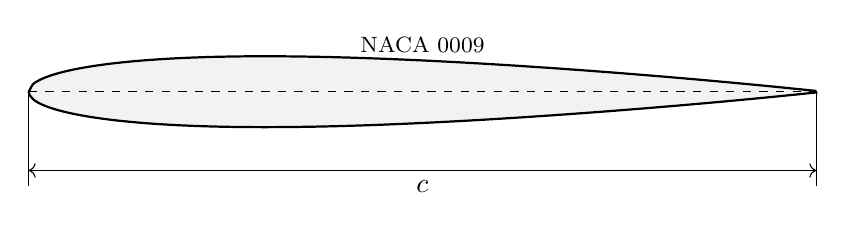
\begin{tikzpicture}[x=10cm, y=10cm]
    % NACA 0009 Equation: y_t = 5*t * (0.2969*sqrt(x) - 0.1260*x - 0.3516*x^2 + 0.2843*x^3 - 0.1015*x^4)
    % t = 0.09
    \draw[thick, fill=gray!10] plot[domain=0:1, samples=200, smooth] (\x, {5*0.09*(0.2969*sqrt(\x) - 0.1260*\x - 0.3516*\x^2 + 0.2843*\x^3 - 0.1015*\x^4)}) -- plot[domain=1:0, samples=200, smooth] (\x, {-5*0.09*(0.2969*sqrt(\x) - 0.1260*\x - 0.3516*\x^2 + 0.2843*\x^3 - 0.1015*\x^4)}) -- cycle;
    
    % Chord Line
    \draw[dashed, thin] (0,0) -- (1,0);
    
    % Annotations
    \draw[<->] (0,-0.1) -- (1,-0.1) node[midway, below] {$c$};
    \draw (0,0) -- (0,-0.12);
    \draw (1,0) -- (1,-0.12);
    
    \node at (0.5, 0.06) {\footnotesize NACA 0009};
\end{tikzpicture}
\end{document}
